\clearpage
\chapter{Appendix}

\section{Horizontal prototype}
\label{horizontal-prototype}

\begin{figure}[h!]
    \centering
    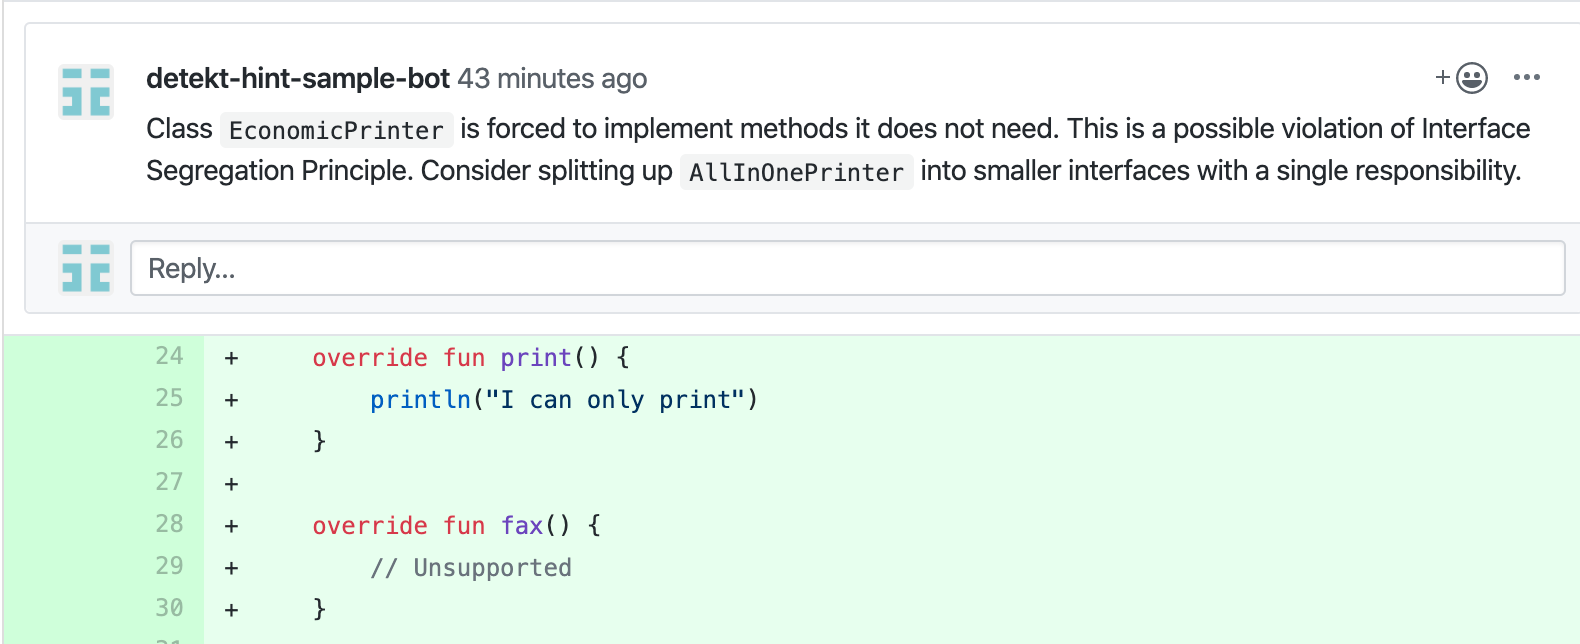
\includegraphics[width=\textwidth]{../images/comment_isp.png}
    \caption{Prototype of the \gls{isp} rule }
    \label{fig:isp}
\end{figure}


\begin{figure}[h!]
    \centering
    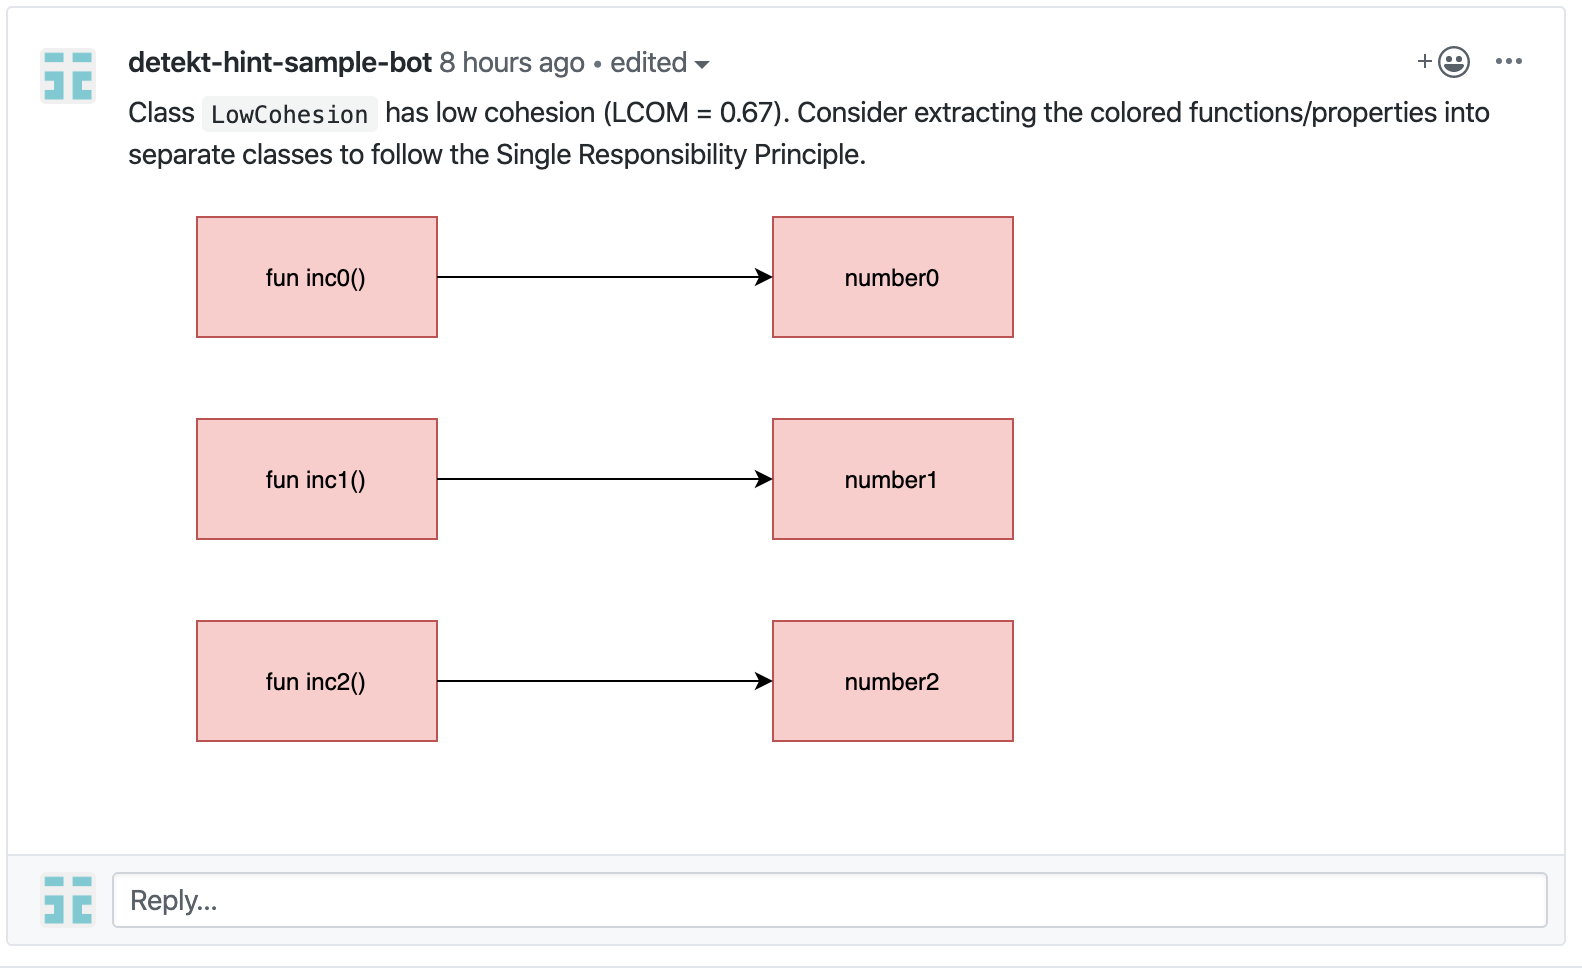
\includegraphics[width=\textwidth]{../images/comment_lackOfCohesion.png}
    \caption{Prototype of the \gls{lcom} rule}
    \label{fig:lcom}
\end{figure}


\begin{figure}[h!]
    \centering
    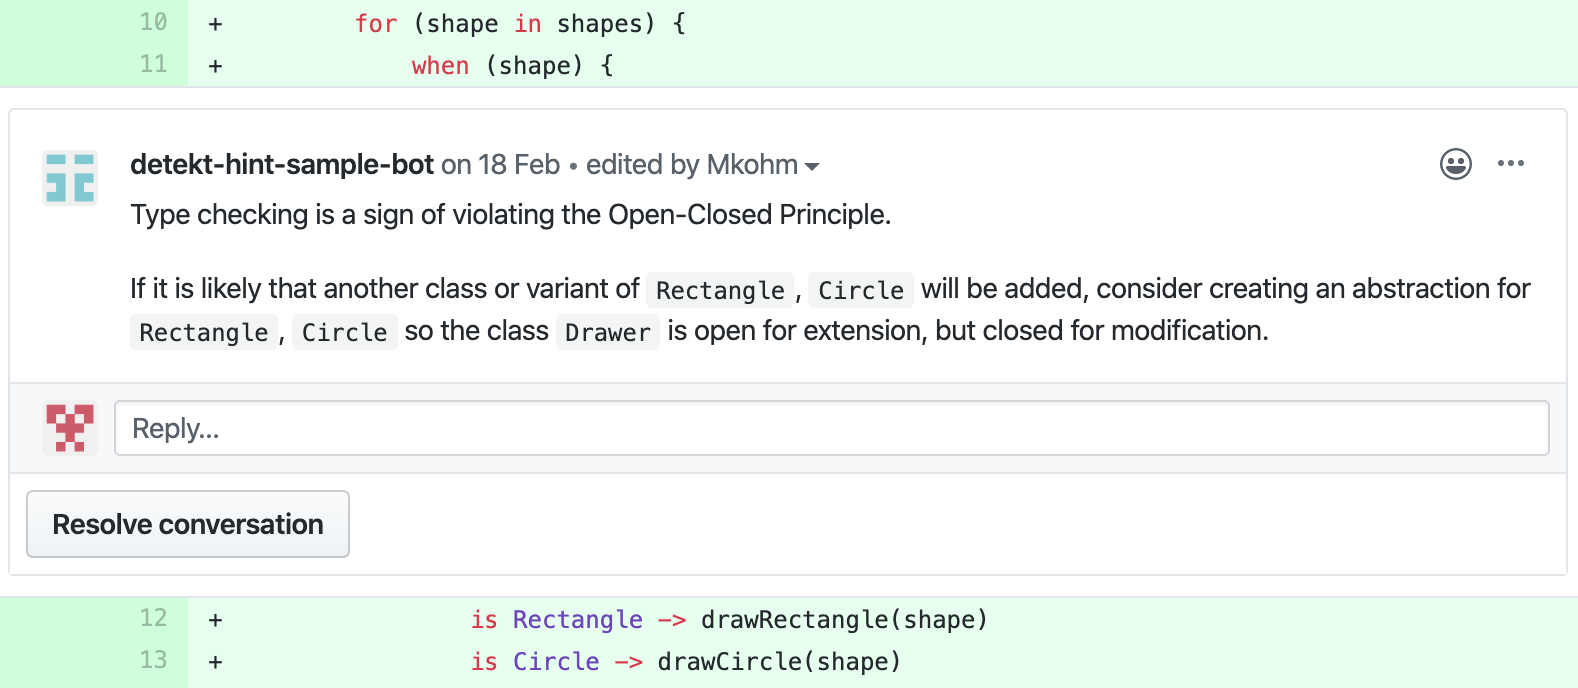
\includegraphics[width=\textwidth]{../images/comment_ocp.png}
    \caption{Prototype of the \gls{ocp} rule}
    \label{fig:ocp}
\end{figure}


\begin{figure}[h!]
    \centering
    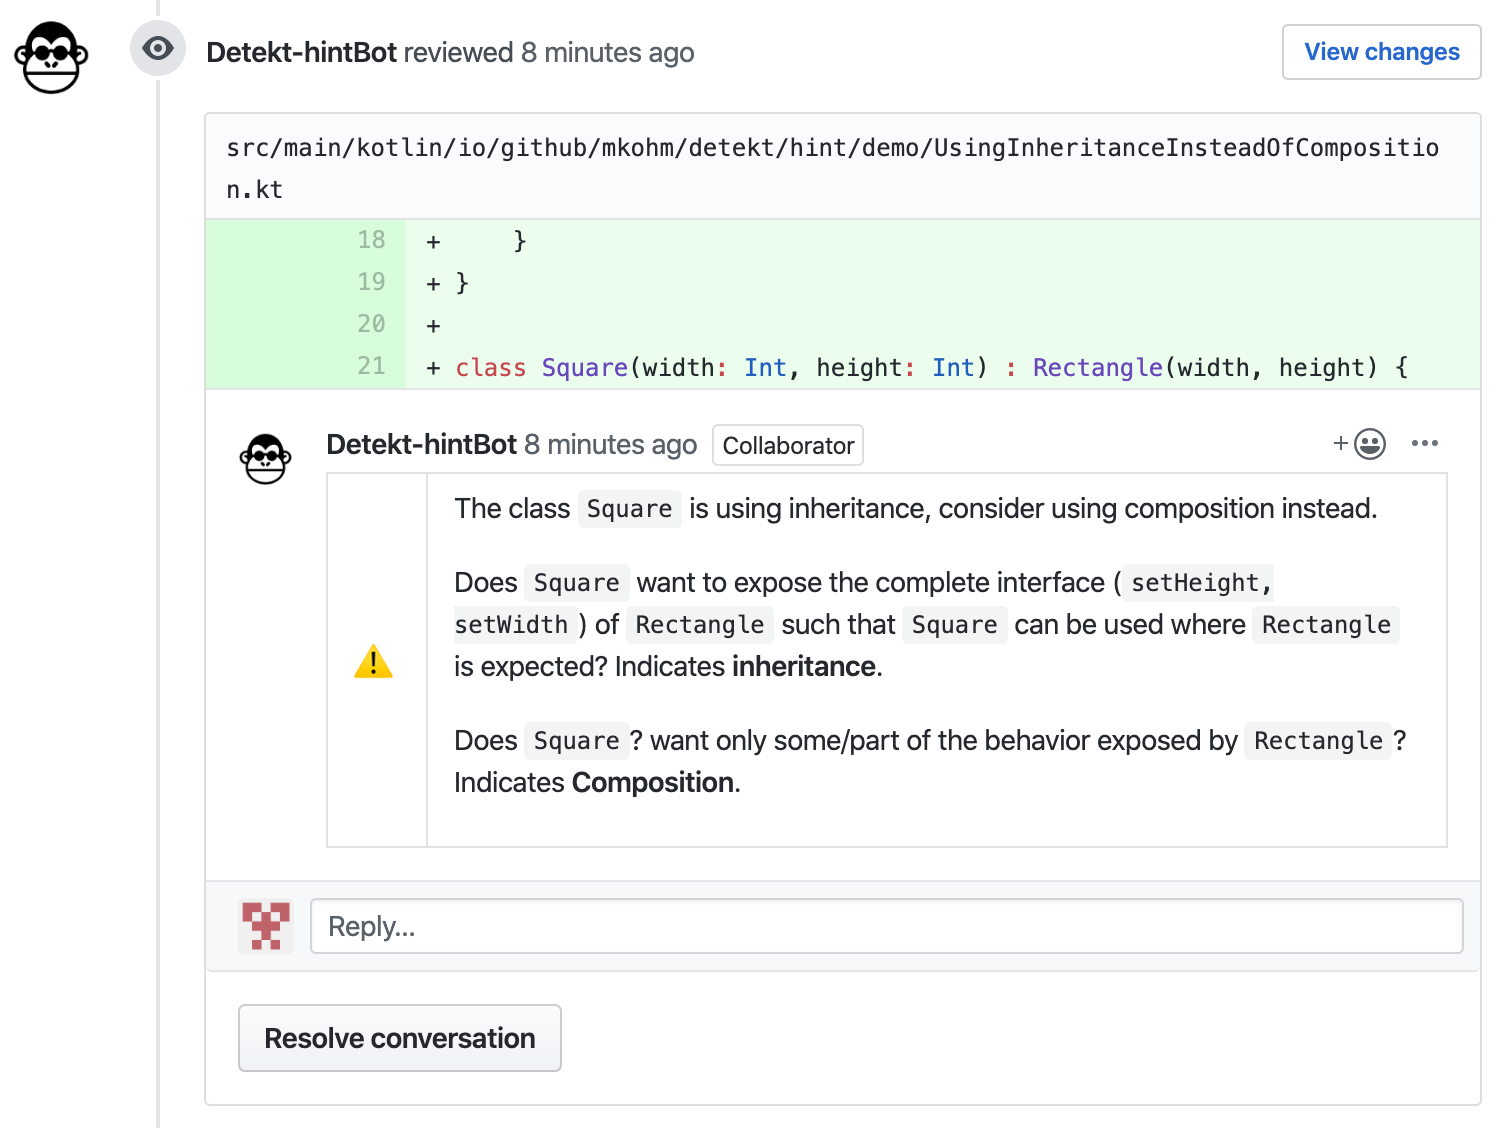
\includegraphics[width=\textwidth]{../images/demo.png}
    \caption{Prototype of the composition over inheritance / \gls{lsp} rule}
    \label{fig:liskov}
\end{figure}

\clearpage

\section{Horizontal prototype schema}
\label{semi-structured-interview-schema}
\subsubsection*{Participant number:} What is the number of the participant.
\subsubsection*{Background:} What is the participants background. Experience with software architecture? Knows and uses design principles? Experience with Kotlin?
\subsubsection*{Presentation of rules - For each rule}
\begin{enumerate}
    \item Present the rule. 
    \item Make sure the participant understands the importance of the rule.
    \item When will the rule give a warning?
    \item When will the rule incorrectly give a warning? Will it report false-positives too often? Suggestions on how to reduce the amount?
    \item How much context is needed? Shorter or longer comments? Should include suggestions on possible solutions? Is the comment understandable? Something missing?
\end{enumerate}

\subsubsection*{Other} 
- When reviewing code, what do you think is tedious, and could it be automated?
- Are there any rules/principles missing?

\clearpage
\section{Horizontal prototype results}
\textbf{Participant number:} 1 \newline
\textbf{Background:} Studies computer science at \gls{ntnu} with a specialization in computers and systems software. Has experience with developing apps for iOS and web and back-end development. Interested in Software Architecture and writing software of high quality. \\
\textbf{Experience with design principles:} Some \\\\

\noindent UseCompositionInsteadOfInheritance: Could be useful, but potentially have too many false positives. For testing Eirik often creates Mock objects that inherits from the class he wants to Mock, and then overrides methods. Eirik think there is too few cases where this rule will be useful. Suggestions: Reduce the amount of positives by disabling checks for classes with names; Mock. User could specify which class names or a pattern to ignore. Should revisit sentence number two about composition, it could be misleading.\\\\

\noindent LCOM1: Very useful because calculating such a value is'nt something you do while coding. Positive that you can change the threshold of the rule. Suggestion: Which fields and methods could i extract? A comment that suggests a solution. \\\\

\noindent LCOM2: Look more at further analysis to find out what can be extracted. Look into dependencies between function calls as well. Diagram looks cool, but does not give any more value than some plain text explaining what can be extracted. \\\\

\noindent OCP: Somewhat useful. Should have a more specific comment saying if you are doing enum switching or instanceOf checking. \\\\

\noindent ISP: Could be useful. Suggestion to count number of usages of calls in the interface to see which method calls that is not used by any of the classes that implement the interface. \\\\

\noindent Other: Tools for detecting complicated expressions that can be extracted out as a separate method with a descriptive name. Blocks of code should be extracted out as separate methods so that lines of code that belongs together has its own scope. 
\clearpage


% Netlight
\noindent\textbf{Participant number:} 2 \newline
\textbf{Background:} Works as a software developer for Netlight, x years of experience with Kotlin.\\
\textbf{Experience with design principles:} Yes \\\\

\noindent UseCompositionInsteadOfInheritance: Positive about the rule, but is concerned about not showing warnings when deriving from third party libraries. This is a case where one also should think about using composition instead of inheritance. Suggests to remove this logic, and instead provide configuration options for packages that should not be reported as violations when derived from.  \\\\

\noindent LCOM: Nothing special. \\\\

\noindent OCP: Useful for both instance of checking and enum switching. Enums in Kotlin are powerful, so switching on them is in many cases not needed and polymorphism is used instead.\\\\

\noindent ISP: Could be useful. May need to handle TODO's specially. \\\\

\noindent Other: In general positive to the tool, and think it has potential. Good that it is easy to ignore warnings, with just a click. It needs more rules before considering using it. For example including detection of Java antipatterns and ensuring that Kotlin code is idiomatic. For example static methods and places where data-classes could be used. The tool could be used as "training wheels" in a team, where one gradually could disable more rules to not create unnecessary noise in the development.
\clearpage

\section{Final artifact}
\begin{figure}
    \centering
    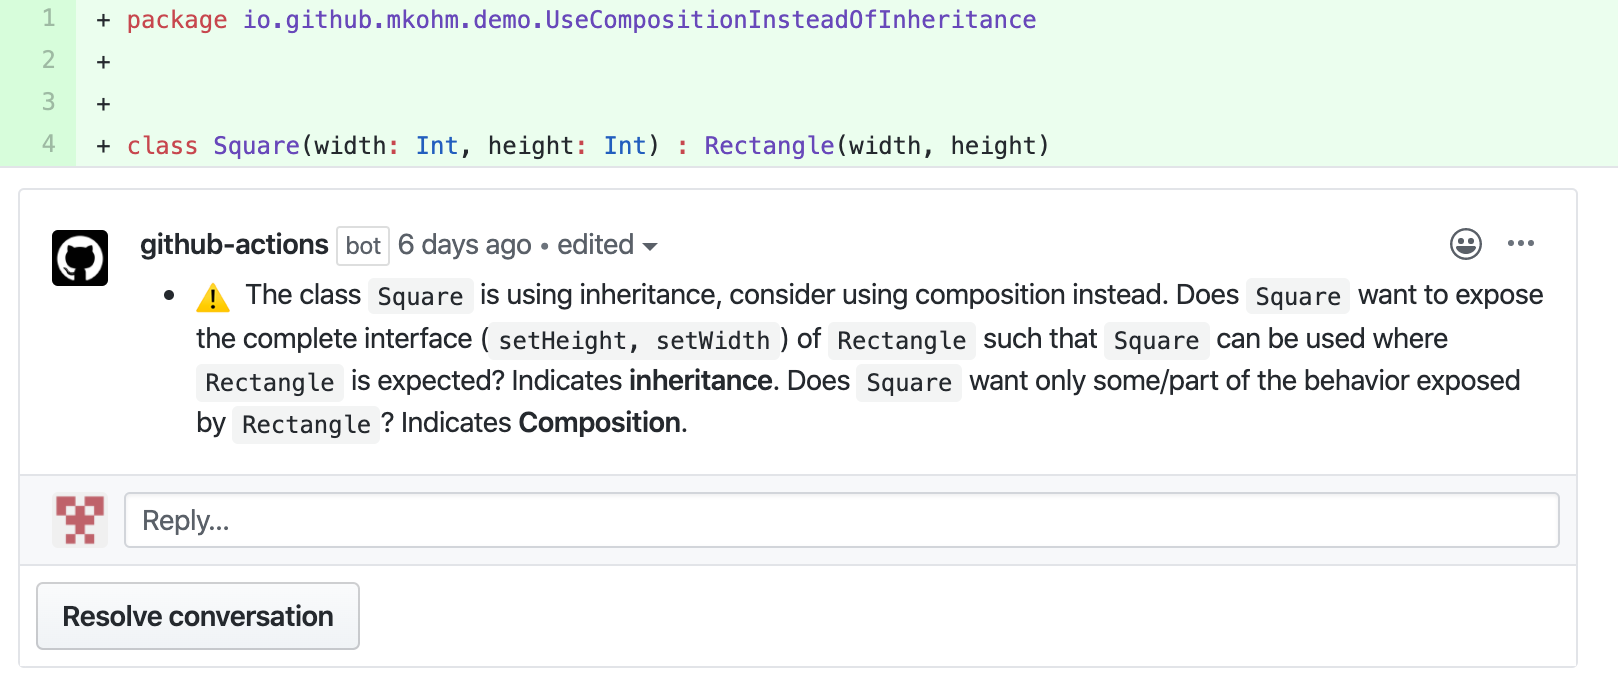
\includegraphics{final_coh.png}
    \caption{Working prototype of \gls{coh}}
\end{figure}

\begin{figure}
    \centering
    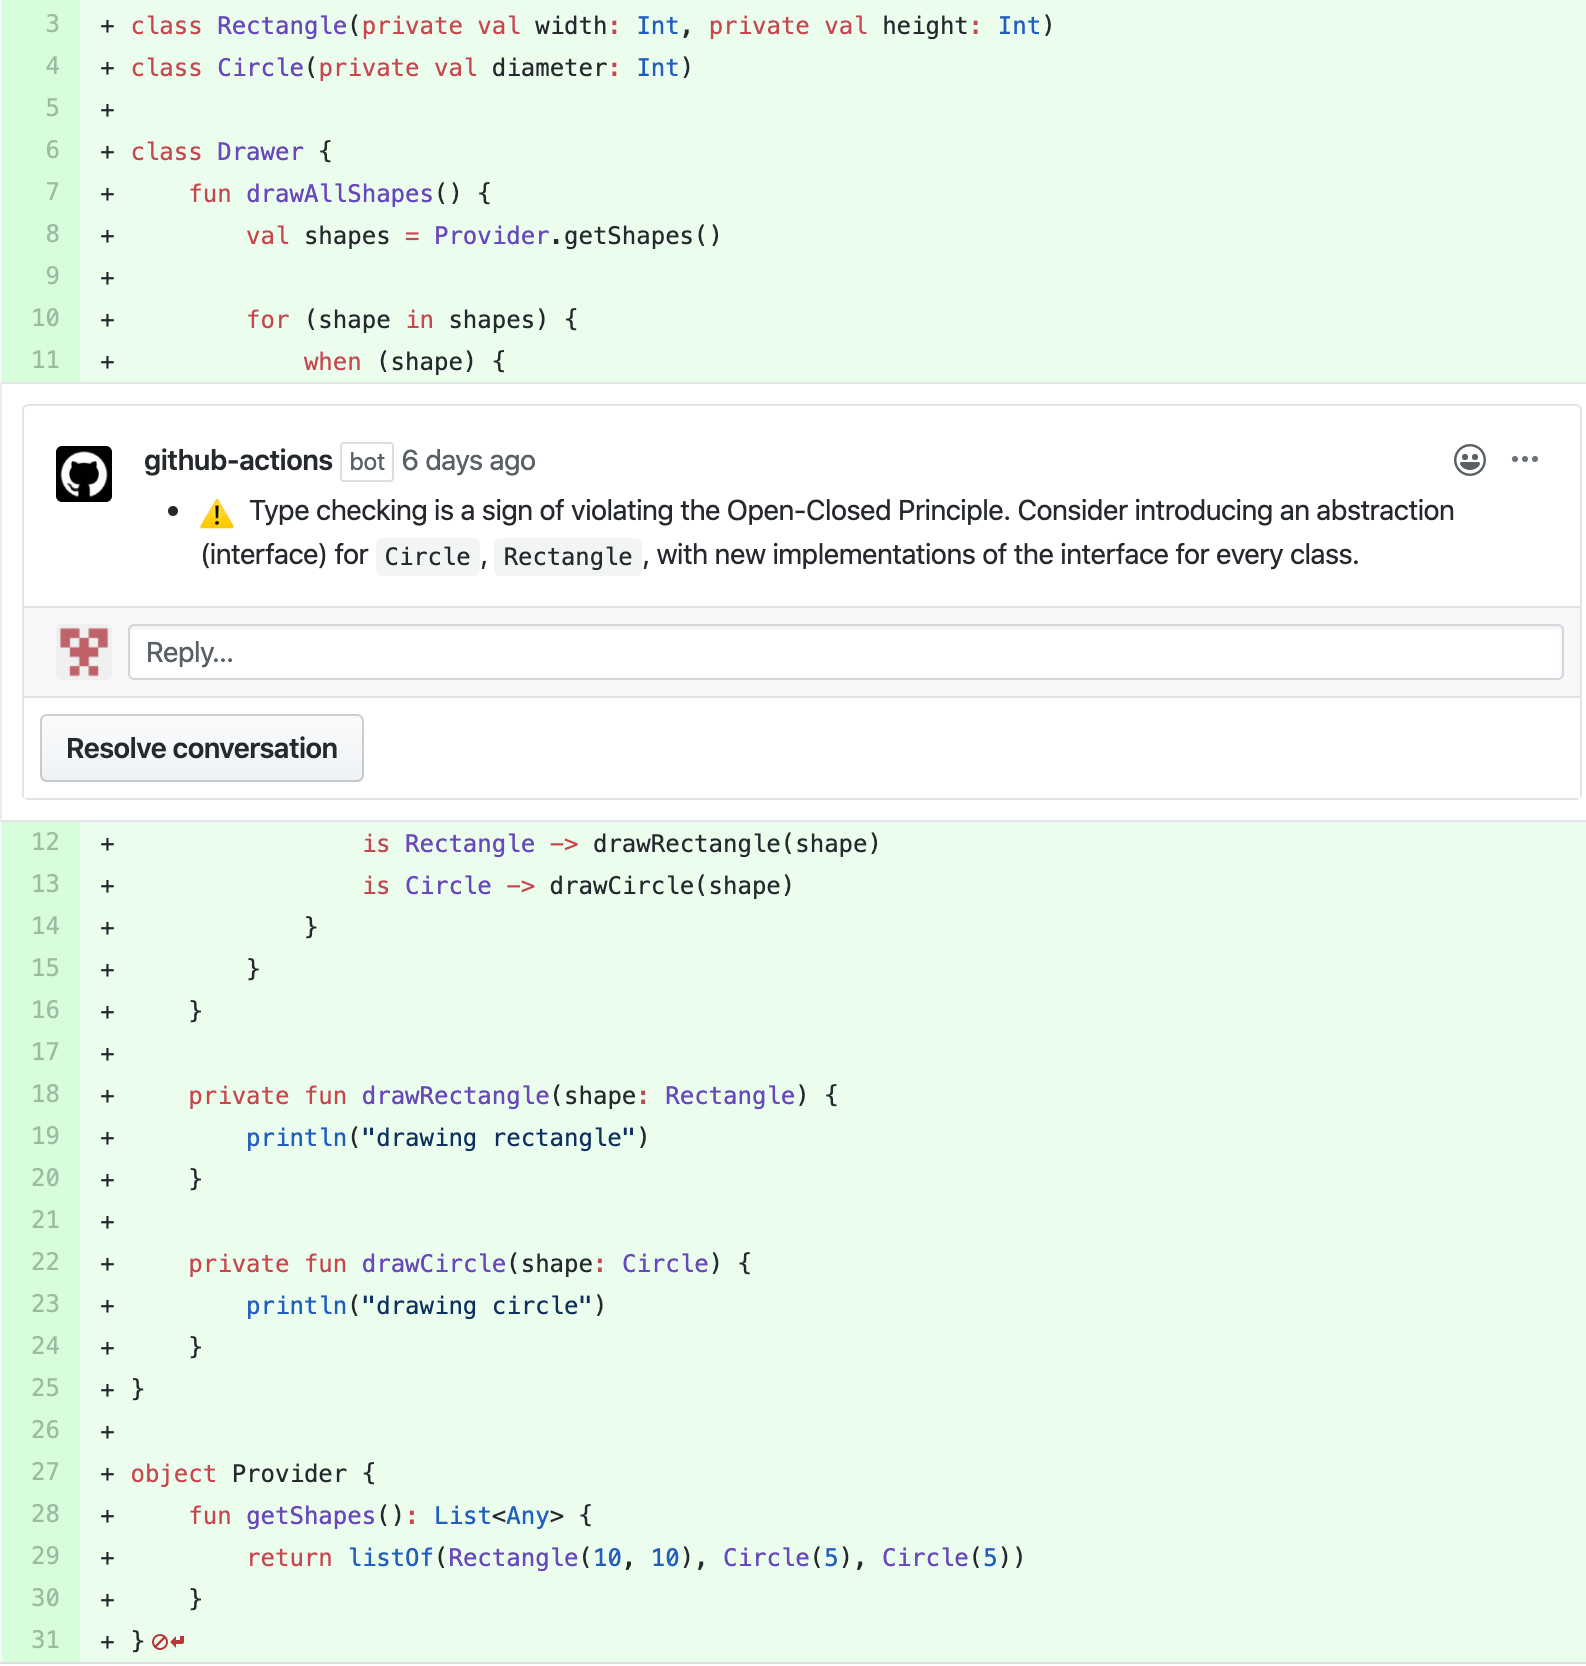
\includegraphics{final_ocp}
    \caption{Working prototype of \gls{ocp}}
\end{figure}

\begin{figure}
    \centering
    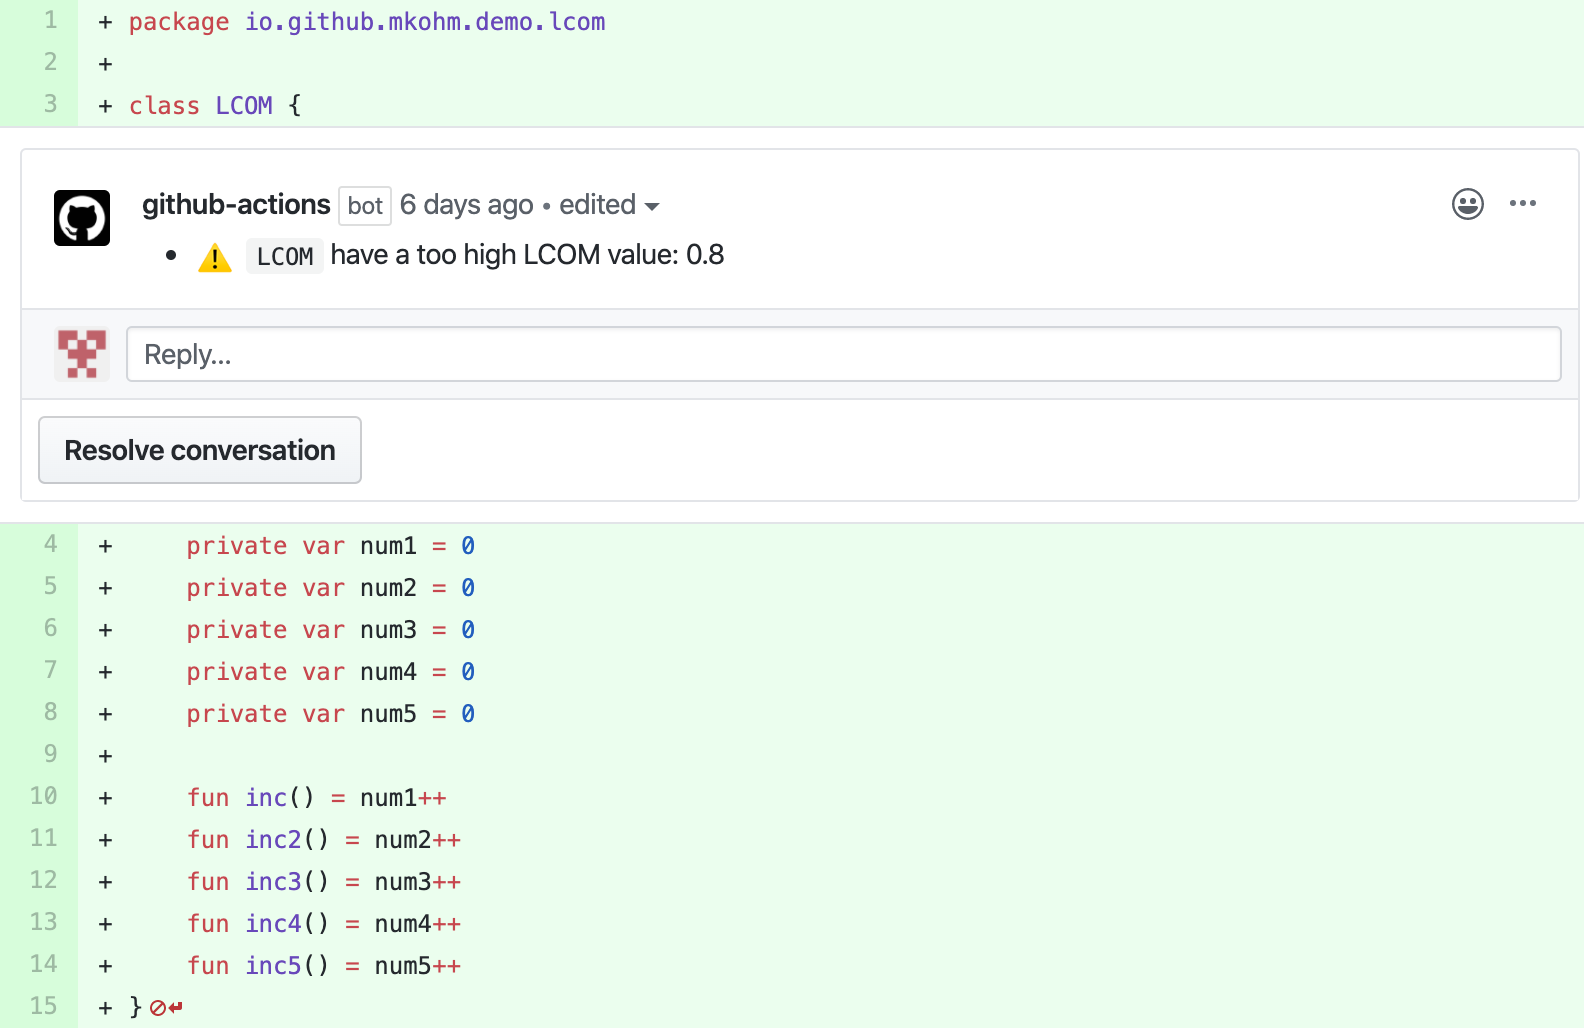
\includegraphics{final_lcom}
    \caption{Working prototype of \gls{lcom}}
\end{figure}

\begin{figure}
    \centering
    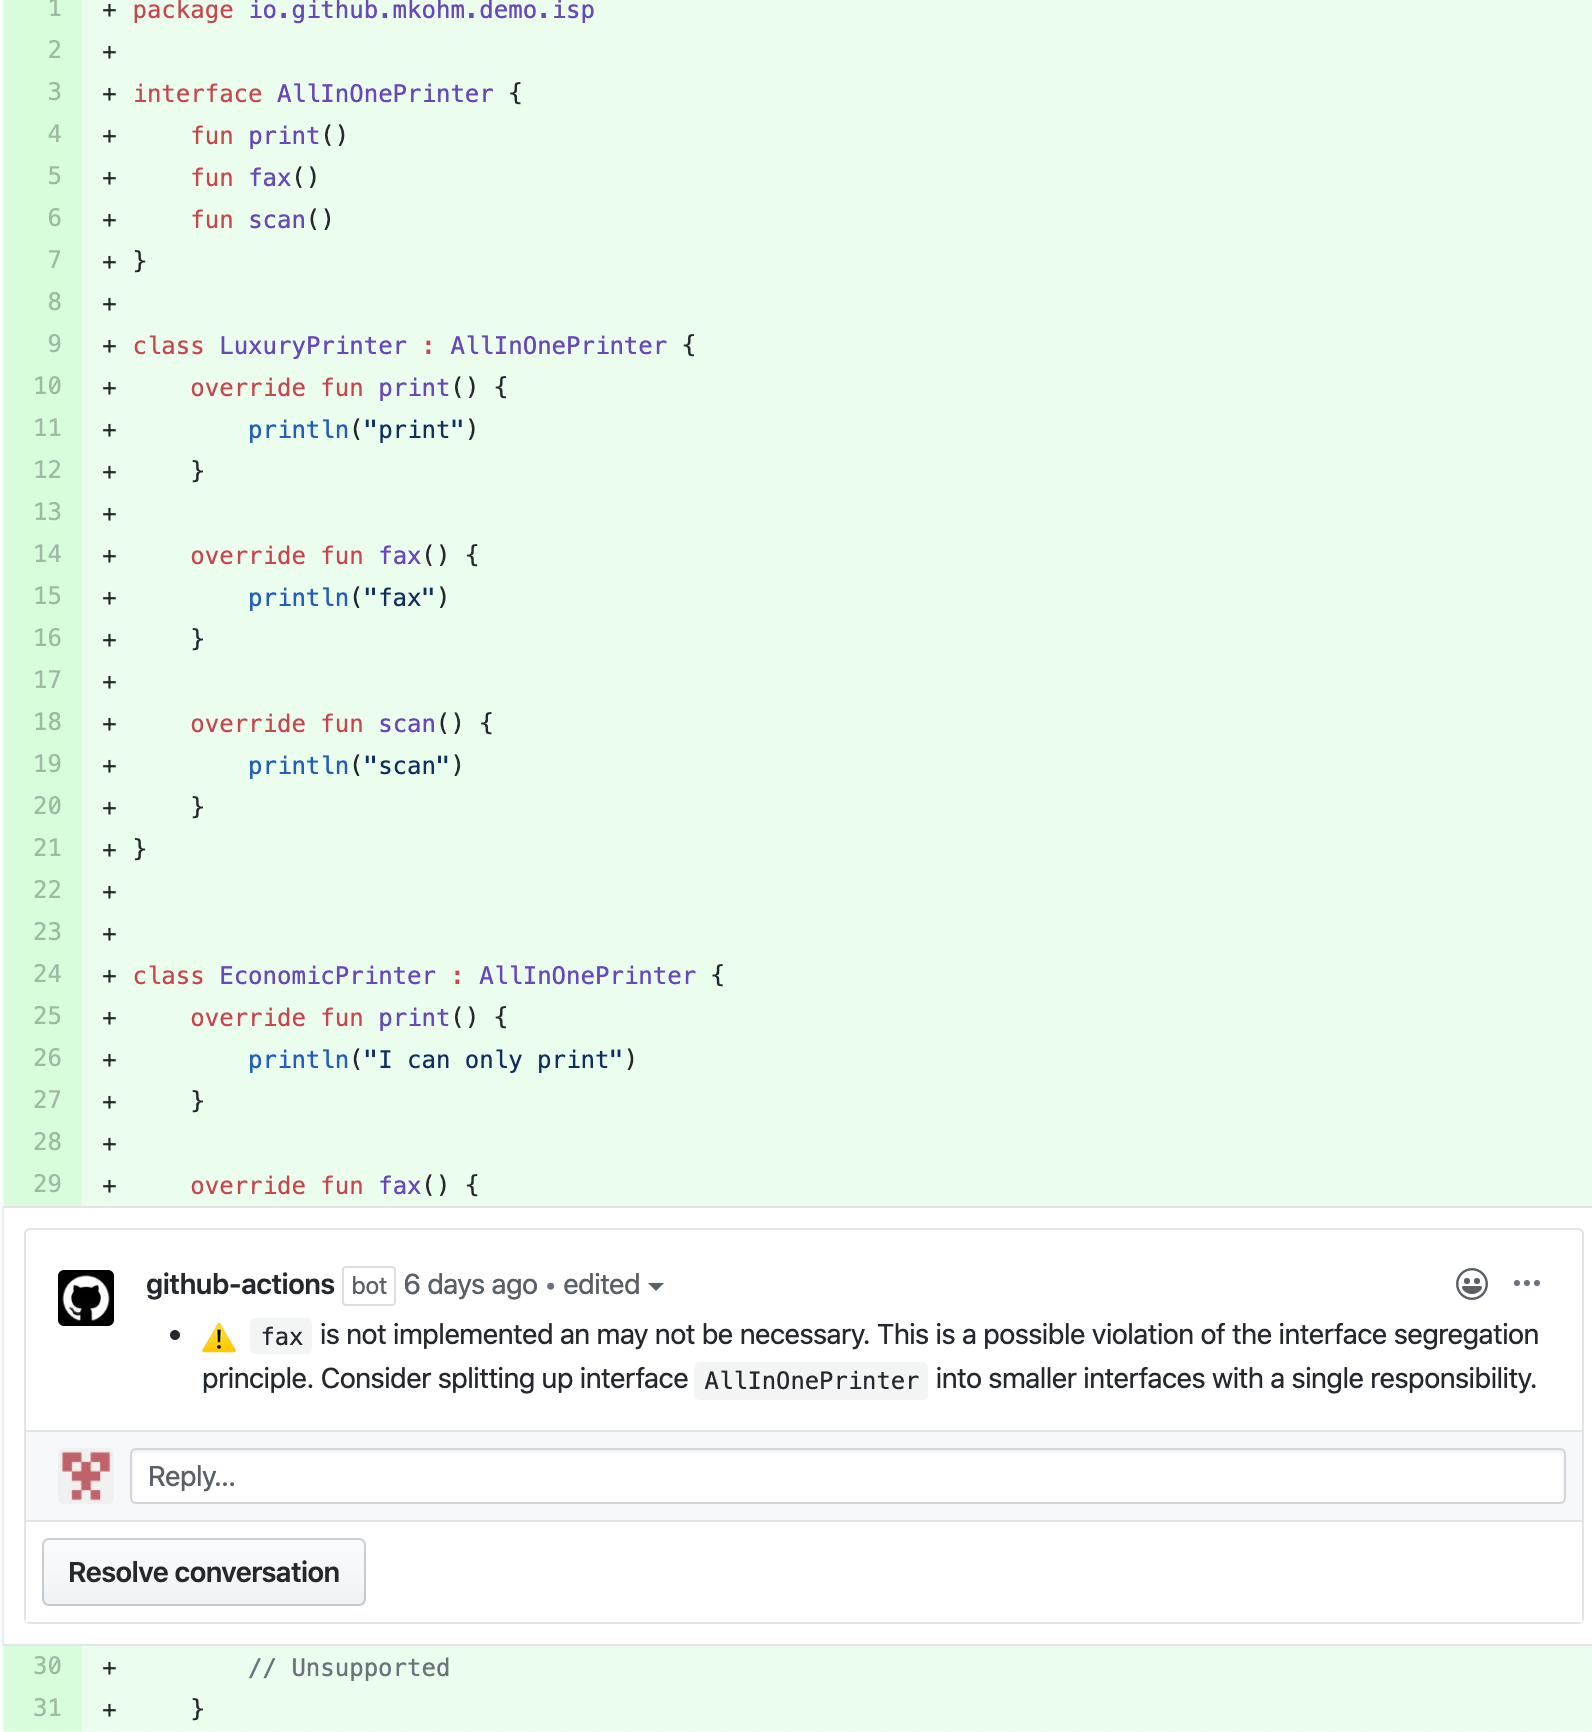
\includegraphics{final_isp}
    \caption{Working prototype of \gls{isp}}
\end{figure}


\todo{Publish pre study somewehere so that i can link to it?}
